%%% Local Variables: 
%%% coding: utf-8
%%% mode: latex
%%% TeX-engine: xetex
%%% End:

% main.tex файл который компилируется и подключает за собой остальный
% файлы с содержимым через input
% При этом согласно моей же логике преамбула должна отстаться здесь.

% Используем опцию emptystyle т.к. bsuir-std расширяет eskdxtext,
% который без этой опции сделает рамку для чертежа даже на документе
% с просто текстом.
\documentclass[a4paper,emptystyle]{bsuir-std}


% BibLaTeX нужен для библиографии
\usepackage[backend=biber,sorting=none]{biblatex}
% Эта штука рекомендуется вместе с biblatex
\usepackage{csquotes}


% Добавляем файл с библиографией
\addbibresource{Karakin5semCoursework.bib}


\begin{document}

% Путь к месту где картинки лежат
\graphicspath{ {images/} }

%%% Титульник
%%% Local Variables: 
%%% coding: utf-8
%%% mode: latex
%%% TeX-engine: xetex
%%% End:

%%% Титульный лист

\begin{titlepage}
  % Устаналиваем стиль ESKD empty, иначе на титульнике будет стоять
  % номер страницы. Потому что в классе bsuir-std я включил нумерацию.
  \ESKDstyle{empty}
  \ESKDthisStyle{empty}
\begin{center}
Министерство образования Республики Беларусь\\[1.2em]
Учреждение образования\\[0.4em]
БЕЛОРУССКИЙ ГОСУДАРСТВЕННЫЙ УНИВЕРСИТЕТ ИНФОРМАТИКИ И РАДИОЭЛЕКТРОНИКИ\\[2.0em]
\end{center}
Факультет компьютерного проектирования\\
Кафедра проектирования информационно-компьютерных систем

\begin{flushright}
  \begin{minipage}{0.5\textwidth}
    \textit{К защите допустить:}\\
    Руководитель курсового проекта\\
    Доцент, к.т.н.\\
    \underline{\hspace*{2.8cm}} Г.\,А.~Пискун
  \end{minipage}\\[2em]
\end{flushright}

\begin{center}
  \textbf{ПОЯСНИТЕЛЬНАЯ ЗАПИСКА}\\
  к курсовому проекту\\
  на тему\\[2.0em]

  \textbf{БЕСПРОВОДНОЙ РОУТЕР АССИМЕТРИЧНОЙ ЦИФРОВОЙ АБОНЕНТСКОЙ ЛИНИИ}\\
\end{center}
\end{titlepage}



%%% Введение.
\begin{center}
\textbf{ВВЕДЕНИЕ}
\end{center}

\par
Беспроводной роутер ассиметричной цифровой абонентской линии — это
устройство предназначенное для предоставления доступа в интернет.
\par
Пользовательские устройства подключаются к роутеру по протоколу
беспроводной связи, а сам роутер включается в сеть интернет-провайдера
по модемной технологии ассиметричной цифровой абонентской линии.
Ассиметричность цифровой абонентской линии означает то, что исходящая
пропускная полоса канала связи может быть не равна входящей.
\par
В данном случае роутер предоставляет доступ в интернет в пределах
одного дома, квартиры или небольшого офиса.
Однако даже для того, чтобы обеспечить работу даже в пределах
небольшой домашней сети, требуются вычислительные ресурсы,
которые используются роутером для выполнения задач
по обеспечению работоспособности сети.
\par
В такие типовые задачи роутера входит:
\begin{itemize}[nosep]

\item Трансляция сетевых адресов;
\item Динамическая конфигурация подключаемых устройств;
\item Фильтрация сетевых пакетов.
\end{itemize}
\par
В результате работы роутер нагревается, а охлаждение этого устройства
является основной темой данной курсовой работы.
\par
Цель данной курсовой работы — обосновать эффективность выбранной
системы охлаждения, для беспроводного роутера ассиметричной цифровой
абонентской линии 68.4 мВт, 12 В, модель ASW800 ADSL.
Задача курсовой работы – провести анализ теплового режима
радиоэлектронного средства в негерметичном перфарированным корпусом,
охлаждаемого с помощью естественной вентиляцией, и на основании
полученных результатов расчетов сделать вывод об эффективности
выбранного метода охлаждения.
\par
В курсовой работе использовались такие методы исследования, как:
\begin{itemize}[nosep]
\item аналитический;
\item физико-математический;
\item метод моделирования и компьютерной обработки данных.  
\end{itemize}

\par
В первом разделе курсовой работы рассматривается и анализируется
устройство и его внутренние компоненты, по которым производится
расчёт теплового режима. Во втором разделе производятся расчеты
теплового режима РЭС и краткий анализ полученных данных.
В третьем разделе описывается процесс модерилования тепловой
картины поля микросхемы РЭС, описывается программный комплекс для моделирования.
В четвертом разделе сравниваются и анализируются данные, полученные при расчете
и определяется адекватность полученных данных.

\newpage

%%% Первая глава
\section{ОБЩЕТЕХНИЧЕСКИЙ АНАЛИЗ ПРОЕКТИРУЕМОГО УСТРОЙСТВА}
\subsection{Анализ исходных данных}
\par
В курсовой работе рассматривается беспроводной роутер асимметричной
цифровой абонентской линии.  Чтобы кратко сформулировать назначение
данного сетевого устройства достаточно одного слова — маршрутизатор.
Потому что именно задачу маршрутизации, то есть доставки сетевых
пакетов из пользовательской сети в сеть интернет-провайдера решают
такого рода устройства.
\par
Одной из функций маршрутизатора является физическогое соединение
сетей. Маршрутизатор имеет несколько сетевых интерфейсов, подобных
интерфейсам компьютера, к каждому из которых может быть подключена
одна сеть. Маршрутизатор может быть реализован программно на базе
универсального компьютера (например, типовая конфигурация Unix или
Windows включает программный модуль маршрутизатора). Однако чаще
маршрутизаторы реализуются на базе специализированных аппаратных
платформ. В состав программного обеспечения маршрутизатора входят
протокольные модули сетевого уровня ~\cite{NetworksOlifer2016}.

Роутер выполнен в виде платы с распаянными компонентами, в
негерметичном корпусе с перфорацией для обеспечения естественной
вентиляции РЭС. Корпус имеет форму параллелепипида, на задней панели
содержит разъём RJ-45 для подключения к телефонной сети и четыре
разъёма для подключения по стандарту Ethernet, антенну, разъём питания
и тумблер включения.

\begin{figure}[h] %% h means here
  \centering
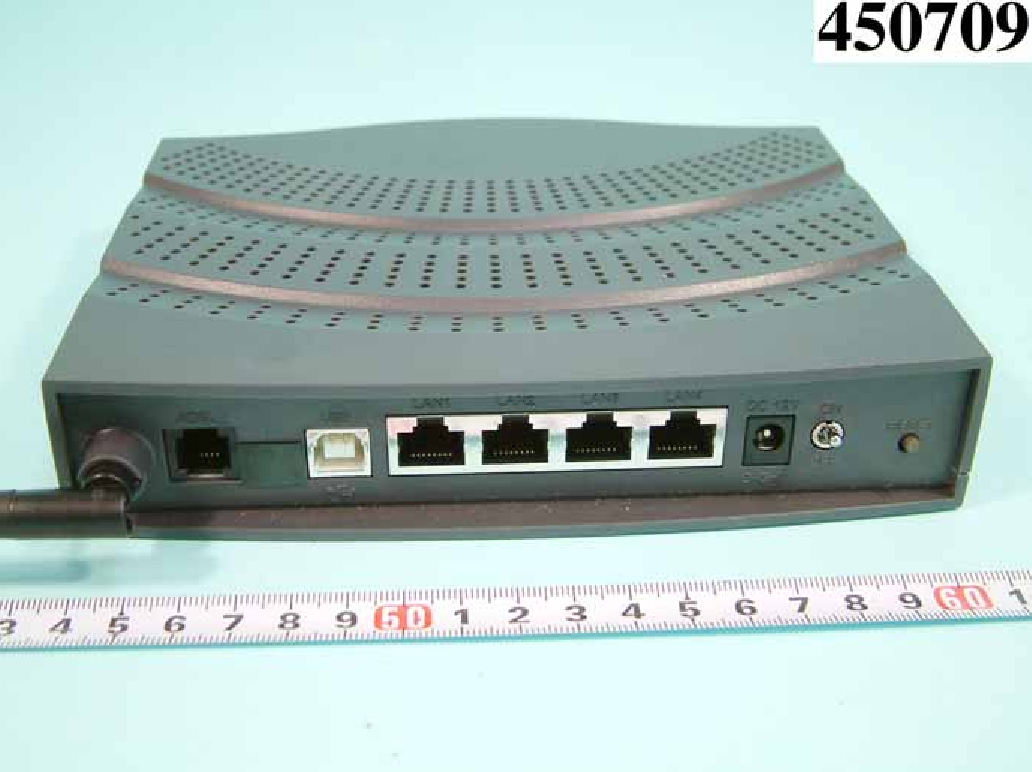
\includegraphics[scale = 0.7]{external_photos-2.png}
\caption{Фотография задней панели роутера ~\cite{EXTERNAL_PHOTOS}.}

\end{figure}

Поскольку в курсовой работе будет производиться расчёт тепловых
режимов будет также важно учитывать климатические факторы внешней
среды, то какие условия эксплутации при этом должны быть соблюдены
регламентирует соответсвующий стандарт — ГОСТ 15150-69
~\cite{GOST_15150-69}.

Настоящий стандарт должен применяться при проектировании изделий.  В
частности, он должен применяться при состалвении технических заданий
на разработку или модернизацию изделий, а также при разработке
государственных стандартов и технических условий, устанавливающих
требования в части воздействия климатических факторов внешней среды
для группы изделий, а при отсуствии указанных групповых документов —
для отдельных видов изделий ~\cite{GOST_15150-69}.

Для конкретных типов или групп изделий виды воздействующих
климатических факторов и их номинальные значения устанавливаются в
зависимости от условий эксплуатации изделий в соответвующих
технических заданих, стандартах и технических условиях ~\cite{GOST_15150-69}.

Так как в данном случае роутер предоставляет доступ в интернет в
пределах одного дома, квартиры или небольшого офиса. Можно говорить, что роутер соответствует категории УХЛ4.2 ГОСТ15150-69.

Характеристика данной категории следующая:\\
Для эксплуатации в помещниях (объемах) с искуственно регулируемыми
климатическими условиями, например в закрытых отапливаемых или
охлаждаемых и вентелируемых производственных и других, в том числе
хорошо вентилиуруемых подземных помещниях (отсуствие воздействия
прямого соленчного излучения, атмосферных осадков, ветра, песка и пыли
наружного воздуха; отсутвие или существенное уменьшение воздействия
рассеяного солнечного излучения и конденсации влаги). Для эксплуатации
в лабораторных, капитальных и других подобного типа помещениях ~\cite{GOST_15150-69}.

Соответствие условий работы роутера ассиметричной цифровой абонетской
линии данному ГОСТ важно по той причине, что климатические условия
регламентиуремые ГОСТ влияют на внешние тепловые воздействия на РЭС.
В зависимости от них также может быть выбран корпус определённого
типа.

\subsection{Описание принципа работы анализируемого устройства}


Рассмотренной устройство — специализированная аппартная платформа,
реализующего фукнции маршрутизатора в сетевой топологии.  Чтобы ещё
больше конкретизировать назначение устройства необходимо упомянуть в
каком сегменте сети оно осуществляет свою работу.


Локальная сеть (LAN, Local Area Network) — частная сеть,
функционирующая в отдельном здании и на прилегающей территории
(это может быть дом, офис или завод). LAN широко применяется для соединения персоналтьны компьютеров и бытовой электроники, позволяя совместно
использовать различные ресурсы (например, принтеры) и обмениваться
информацией ~\cite{NetworksTanenbaum2023}.

На сегодняшний день беспроводные LAN применяются
повсеместно. Изначально они были популярны в жилых помещениях, старых
офисных зданиях, кафе и других местах, где прокладка кабелей обошлась
бы слишком дорого. В подобных система компьютеры обмениваются
информацией с помощью встроенного радиомодема и антенны. Чаще всего
компьютер обращается к специальному устройству, которой называется
точкой доступа (AP, Access Point), беспроводным маршрутизатором
(wireless router) или базовой станцией (base station). Это устройство
осуществляет передачу пакетов данных между беспроводными компьютерами,
а также между компьютером и интернетом. Точка доступа напоминает
популярного ребенка в школе, поскольку все хотят с ней «поговорить»
~\cite{NetworksTanenbaum2023}.

Одним из самых популярных стандартов беспроводных LAN является IEEE
802.11, более известный как wi-fi ~\cite{NetworksTanenbaum2023}.

И именно этому стандарту следует рассматриваемое устройство.

Вместо дорогостоящих лицензируемых частот системы 802.11 работают на
нелицензируемых полосах частот, например ISM («Industrial, Scientific,
and Medical» — «промышленные, научные и медицинские») устанавливаемых
МСЭ-R (например 902-928 МГц, 2,4-2,5 ГГц, 5,725-5,825 ГГц).  Этот
диапазон частот разрешено использовать любым устройствам, но мощность
их излучения должна быть ограничена, чтобы различные устройства не
мешали друг другу. Конечно, из-за этого 802.11-передатчики иногда
начинают конкурировать за частоты с беспроводными телефонами,
системами дистанционного открывания дверей гаража и микроволновками.
Так что до тех пор, пока пользователям не понадобиться позвонить
гаражным дверям, важно все настроить
правильно ~\cite{NetworksTanenbaum2023}.

Таким образом рассмотренное устройства это РЭС основная задача
которого — это прием, модуляция, обработка и передача сигнала другим
устройствам и аппаратуре. При этом, поскольку устройство производит не
только физическую передачу данных, но и коммутацию сетевых пакетов,
оказываются нужными некоторые вычислительные ресурсы.
Следовательно для того чтобы осуществлять вычисления устройство будет
оснащенно микропроцессором.

\subsection{Анализ элементной базы устройства}

Используя блок схему рассмотрим элементную базу
маршрутизатора.


\begin{figure}[h] %% h means here
  \centering
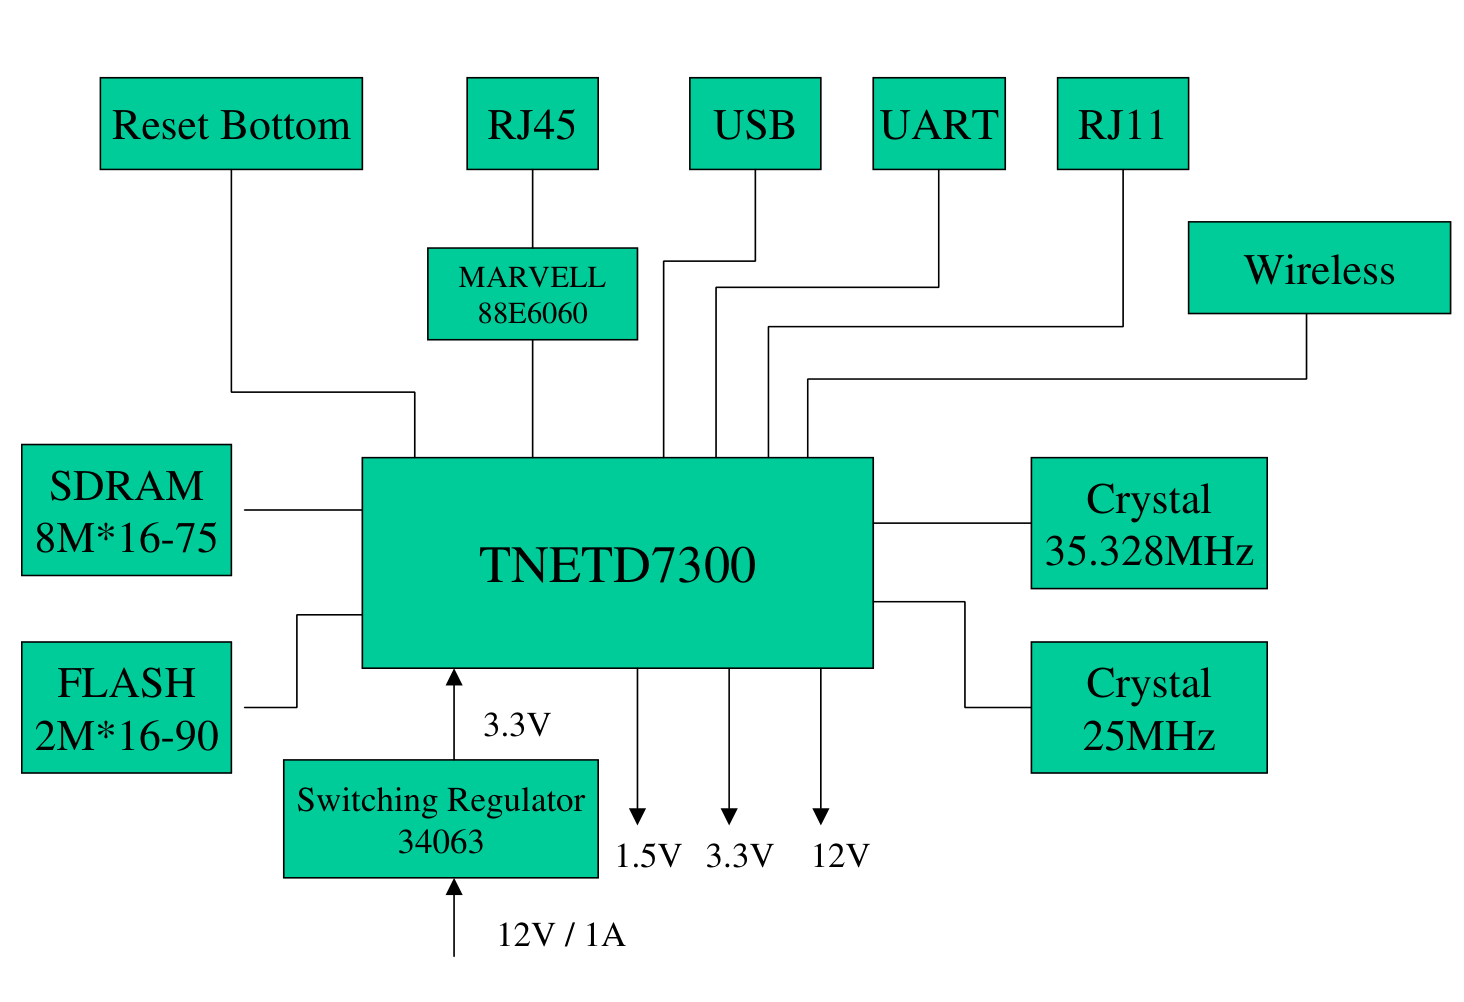
\includegraphics[scale = 0.7]{block_diagram-0.png}
\caption{Блок схема устройства маршрутизатора ASW800ADSL ~\cite{BLOCK_DIAGRAM}.}
\end{figure}
 
Как видно из блок схемы первостепенным и самым важным модулем данной
РЭС явяляется чип TNETD7300, он расположен в цетрне блок схемы. С ним
соеденены несколько интерфейсов и остальные модули.

Из того как расположен этот модуль на блоксхеме можно сделать вывод,
что в этой части РЭС будет рассеиваться больше всего мощности.

Различают внтуренние и внешние тепловые воздействия на РЭА.
Внутренние тепловые воздействия на РЭА в основном зависят от мощности
рассеиваемой её элементами ~\cite{Rotkop1976}.

Энергетический коэффициент полезного действия радиоэлементов, как
правило, невелик, и значительная доля энергии питания превращается в
тепловую энергию с сопутствующим перегревом элементов и аппаратуры
~\cite{Rotkop1976}.

Насыщение современных технических устройств РЭА различного назначения
заставляет конструкторов уменьшать ее габариты и увеличивать удельные
мощности рассеивания, т.е. мощности, приходящиеся на единицу
поверхности или объема РЭА. Одним из основных направлений в
конструировании РЭА стала комплексная микроминиатюризация, что
приводит к ещё большему увелечению удельной мощности рассеивания
~\cite{Rotkop1976}.

%% \pagebreak
Рассмотрим схему электрическую принципиальную на которой изображён чип
TNETD7300.

\begin{figure}[hb]
  \centering
  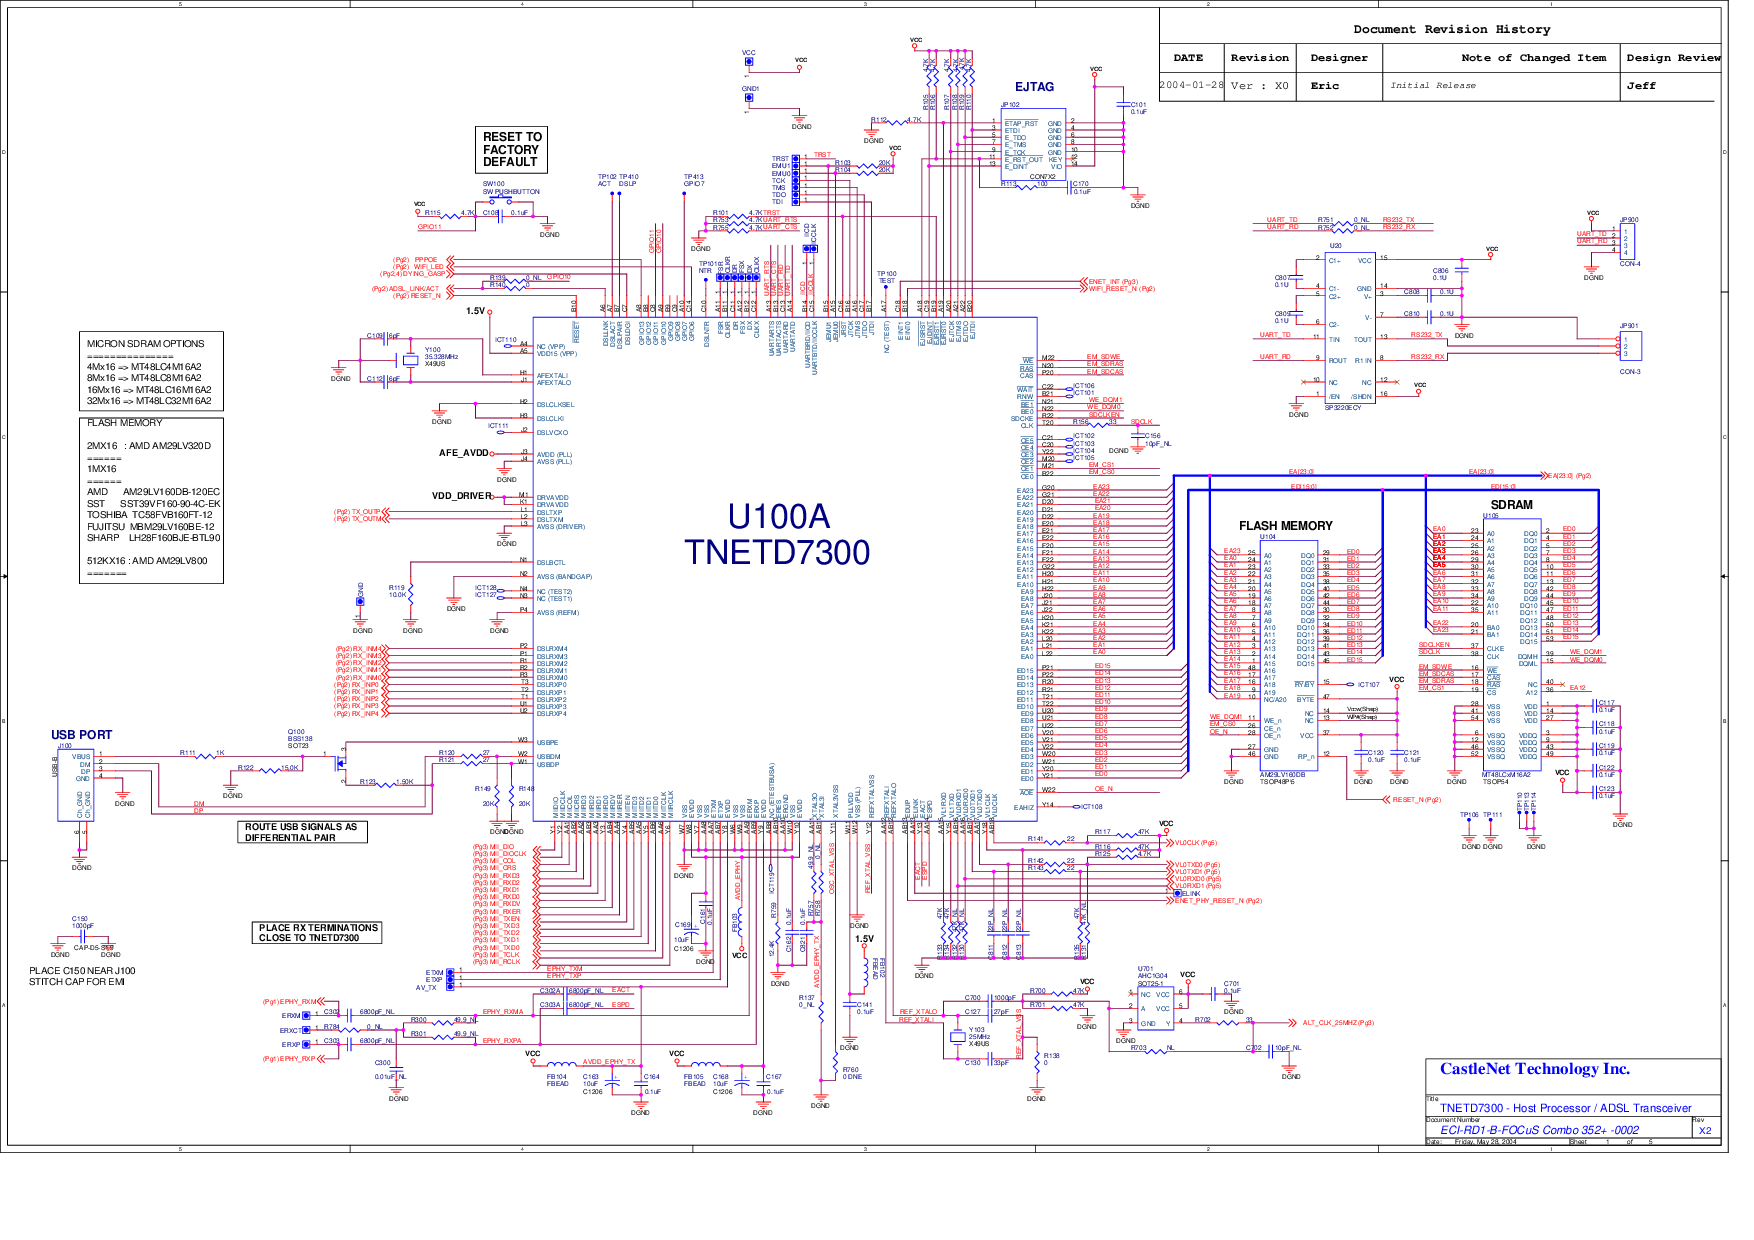
\includegraphics[scale = 0.25]{schematics-1.png}
  \caption{Схема электрическая принципиальная
    маршрутизатора ASW800ADSL ~\cite{SCHEMATICS}.}
\end{figure}

На схеме чип TNETD7300 подписан не иначе как \textit{«Host Proccessor»}.
Из этого можно сделать вывод, что, уже упомянутым в предыдущем
параграфе, микропроцессором и будет являться этот чип.  На схеме
электрической принципиальной микропроцессор выглядит как квадрат к
которому подведены другие компоненты. Такой способ изображения вызван
тем, что для того чтобы показать все элементы из которых состоит
процессор требуется отдельная большая подсхема, которая в свою очередь
была бы разделена на несколько других подсхем соответствующих
отдельным частями процессора, таким как арифметико логическое
устройство, блок управления памятью и другие. Это ещё раз подтверждает
вывод о том, что данное устройство рассеивает больше всего мощности, а
значит и требует наибольшего охлаждения.

\subsection{Выбор и обоснование системы охлаждения}

Защита от тепловых воздействий это одна из важных задач решаемых в обеспечении недёжности РЭС.

Защита РЭА от тепловых воздействий осуществляется при помощи ряда мероприйтий. Одним из основных является использование систем обеспечения теплового режима РЭА (СОТР). СОТР обычно предназначена для поддержания заданного в технических условиях (ТУ) диапазона температур на элементах РЭА, чтобы обеспечить ее надежность при определенных тепловых воздействиях и других специальных требованиях ~\cite{Rotkop1976}.

В радиоэлектронных комплексах СОТР, как правило, являются сложными
системами, состоящими из многих элементов, коммуникациий и несущих
конструкий. В некоторых случаях регулирование температуры в РЭА может
быть достигнуто за счет простейших конструктивных решений,
осущствляющих теплопередачу между элементами РЭА, элементами несущей
конструкции и окружающей средой. Тогда нет смысла рассматривать СОТР
как отдельное изделие и мы будем пользоваться терминами «методы (или
спосбы) охлаждения РЭА». Этими же терминами будем пользоваться и при
исследовании температурного поля элементов РЭА, в результате действия
некоторых гипотетических СОТР, когда конкретная конструкция СОТР не
рассматривается ~\cite{Rotkop1976}.

Для выбора и обоснование системы охлаждения важно иметь представление
о тепловом режиме РЭС.
Тепловой режим есть совокупность значений температур в различных
точках всей РЭС, её корпуса и СОТР.



%%% Вторая глава по разделам
% \section{Расчет теплового режима РЭС при естественном воздушном охлаждении.}
%% 4.2

Расчет теполового режима радиоэлектронных аппартов рекомендуется
проводить в три этапа~\cite{Rotkop1976}:
\begin{enumerate}[label={\arabic*.}]
  \item Определение среднеповерхностной температуры платы с
расположенными ней деталями, корпуса и температуры воздуха внтури
радиоэлектронного аппарата.
  \item Определить среднеповерхностные температуры корпусов элементов
  используя результаты первого этапа.
  \item Определить максимальные температуры критических зон элементов и
их функциональные связи со среднеповерхностной температурой как
корпусов, так и и плат.
\end{enumerate}

Первый и второй этапы расчета позволяют получить значения основных
параметров, связанных с выбором системы охлаждения, т.е. первых двух
этапов хватает для принятия конструкторсого решения касаемо выбора
системы охлаждения.

Полную систему уравнений теплообмена для реального аппарата часто
невозможно не только решить аналитически, но и строго записать. В
связи с этим процессы, протекающие в реальном радиоэлектронном
аппарате, схематизируют, принимают ряд упрощающик предпосылок и в
результате получают тепловую модель аппарата, для которой и проводят
рассчет теплового режима ~\cite{Rotkop1976}.

Наибольшее распространение получила весьма плодотворная схематичзация
процессов теплообмена в РЭА, предложенная Г.Н.Дульневым
~\cite{Dulnev1968}.

Суть метода заключается в том, что печатная плата с её элементами
принимается за одно тело с изотермической поверхностью (нагретую
зону), для которого и проводится расчет теплового режима.

Таким образом производится расчет среднеповерхностной температуры
нагретой зоны.

Под понятием нагретая зона понимается поверхность того элемента на
печатной плате, который рассеивает больше всего мощности.

В данном случае им является процессор ТNETD 7300.

В указанных ранее источниках нет инфомации о том каковы размеры это
чипа. Однако согласно буклету производителя данный чип принадлежит к
вычислительной архитектуре RISC MIPS 32 ~\cite{AR7_fact_sheet}.

Понимание того, к какой архитектуре относится процессор позволяет
определить чипсет, который им используется. В свою очередь данные о
чипсете позволяют сделать вывод о том какова площадь процессора.

Чипсет, размещаемый на материнской плате, выполняет функцию связующего
компонента (моста), обеспечивающего взаимодействие центрального
процессора (ЦП) c различными типами памяти, устройствами ввода-вывода,
контроллерами, как непосредственно через себя, так и через другие
контроллеры и адаптеры, с помощью многоуровневой системы
шин~\cite{Avdeev2019}.

Без чипсета процессор не сможет взаимодествовать с переферийными
устройствами напрямую.

Исходя из даты изготовления всей РЭС и архитекутры конкретного чипа,
можно сделать вывод, что процессор размещается на чипсете R8000
~\cite{R8000_physical_wikipedia}.

Согласно этим данным чипсет имеет форму прямоугольника со сторонами в
$l_1$ = 17,34 мм и $l_2$ = 17,30 мм (занимает площадь 299,98 мм$^2$) и
рассеивает 13 ват мощности.

Основываясь на информации о процессорах тех лет, примем высоту чипа
$l_3$ равной 2,5 мм ~\cite{MobilePentium3_wikipedia}.

Таким образом можно найти условную поверхность нагретой зоны по
формуле:

\begin{equation}
S \mathrm{_з} = 2 (l_1 l_2 + (l_1 + l_2) l_3 K \mathrm{_з} )
\end{equation}

\subsection{Расчет теплового режима РЭС в герметичном корпусе}
%% 4.2.1

\subsection{Расчет теплового режима РЭС в герметичном корпусе с внутренним перемешиванием}
%% 4.2.2.

\subsection{Расчет теплового режима РЭС в герметичном корпусе с наружным обдувом}
%% 4.2.3.

\subsection{Расчет теплового режима РЭС в герметичном оребрённом корпусе}
%% 4.2.4

\subsection{Расчет теплового режима РЭС в перфорированном корпусе}
%% 4.2.5

\subsection{Расчет теплового режима РЭС при принудительном охлаждении}%% 4.2.6

\section{Расчет теплового режима РЭС при естественном воздушном охлаждении.}
\subsection{Расчет теплового режима РЭС в герметичном корпусе}
\begin{enumerate}[label={\arabic*.}]
  
\item Рассчитывается поверхность корпуса блока~\cite{Rotkop1976}:

  \begin{equation}
S\mathrm{_{К}} = 2 \cdot \left(l_1 l_2 + \left(l_1+ l_2 \right)l_3\right) % (4.46)
  \end{equation}

  $$S\mathrm{_{К}}=0,0424\mathrm{м^2}$$

\item Определяется условная поверхность нагретой зоны ~\cite{Rotkop1976}:

  \begin{equation}
    S\mathrm{_{з}} = 2 \left(l_1 l_2 + \left(l_1 + l_2\right) K\mathrm{_{з}} l_3 \right) % (4.39)
  \end{equation}

  $$S\mathrm{_{з}} = 0,03088\mathrm{м^2}$$

\item Определяется удельная мощность корпуса по блоку ~\cite{Rotkop1976}:

\begin{equation}
  q\mathrm{_к} = P\mathrm{_з}/S\mathrm{_к} % (4.45)
\end{equation}

$$q\mathrm{_к} = 306,6037\mathrm{Вт/м^2}$$

\item Рассчитывается удельная мощность нагретой зоны ~\cite{Rotkop1976}:
  \begin{equation}
      q\mathrm{_з} = P\mathrm{_з}/S\mathrm{_3} % (4.38)
    \end{equation}

    $$q\mathrm{_з} = 420,984 \mathrm{ Вт/м^2}$$

\item Находится коэффициент $\vartheta_1$ в зависимости от удельной мощности корпуса блока ~\cite{Rotkop1976}:
    
\begin{equation}
\vartheta_1 = 0,1472q\mathrm{_к} - 0,2962 \cdot 10^{-3}q\mathrm{_к}^2 + 0,3127 \cdot 10^{-6}q\mathrm{_к}^2
\end{equation}

$$\vartheta_1=17,31693$$

\item Находится коэффициент $\vartheta_2$ в зависимости от удельной мощности нагретой среды ~\cite{Rotkop1976}:

\begin{equation}
\vartheta_2 = 0,1390q\mathrm{_к} - 0,1223 \cdot 10^{-3}q\mathrm{_к}^2 + 0,0698 \cdot 10^{-6}q\mathrm{_к}^3
\end{equation}

$$\vartheta_2= 42,04966$$

\item Коэффициент $K\mathrm{_{Н1}}$ в зависмости от давления
  среды вне корпуса блока берётся из ГОСТ~\cite{GOST-15150-69}.

  $$K\mathrm{_{Н1}} = 0,999$$

  \item Коэффициент $K\mathrm{_{Н2}}$ в зависмости от давления
  среды внутри корпуса блока берётся из ГОСТ~\cite{GOST-15150-69}.

  $$K\mathrm{_{Н2}} = 0,996$$

\item Определяется перегрев корпуса блока ~\cite{Rotkop1976}:
  \begin{equation}
    \vartheta\mathrm{_к} = \vartheta_1 \cdot K\mathrm{_{Н1}}
  \end{equation}
  
  $$\vartheta\mathrm{_к} = 17,3 K$$

\item Рассчитывается перегрев нагретой зоны ~\cite{Rotkop1976}:
    \begin{equation}
    \vartheta\mathrm{_з} = \vartheta\mathrm{_к} + (\vartheta_2 - \vartheta_1) \cdot K\mathrm{_{H2}}
    \end{equation}

    $$\vartheta\mathrm{_з} = 41,93 K$$

  \item Определяется средний перегрев воздуха в блоке ~\cite{Rotkop1976}:
        \begin{equation}
      \vartheta\mathrm{_в} = 0,5 \cdot (\vartheta\mathrm{_к} + \vartheta\mathrm{_з})
    \end{equation}

    $$\vartheta\mathrm{_в} = 2,323 K$$

  \item Определяется удельная мощность элемента ~\cite{Rotkop1976}:
    \begin{equation}
      q\mathrm{_{эл}} = \frac{P\mathrm{_{эл}}}{S\mathrm{_{эл}}}
    \end{equation}

        $$q\mathrm{_{эл}} =1109,50966\mathrm{ВТ/м^2} $$

 \item Рассчитывается перегрев поверхности элемента ~\cite{Rotkop1976}:
 \begin{equation}
\vartheta\mathrm{_{эл}} = \vartheta\mathrm{_{з}} \left(a + b \frac{q\mathrm{_{Эл}}}{q\mathrm{_{з}}}\right)
\end{equation}

$$\vartheta\mathrm{_{эл}} =59,079K$$

\item Рассчитывается перегрев окружающей элемент среды ~\cite{Rotkop1976}:

      \begin{equation}
      \vartheta\mathrm{_{эс}} = \vartheta\mathrm{_в}(0,75 + 0,25\frac{q\mathrm{_{эл}}}{q\mathrm{_{з}}})
    \end{equation}
    $$\vartheta\mathrm{_{эс}} = 41,726K$$

  \item Определяется температура корпуса блока ~\cite{Rotkop1976}:
    \begin{equation}
      T\mathrm{_к} = \vartheta\mathrm{_{к}} + T\mathrm{_с}
    \end{equation}
    $$T\mathrm{_{к}} = 330,3 K$$
    
\item Определяется температура нагретой зоны ~\cite{Rotkop1976}:
    \begin{equation}
      T\mathrm{_з} = \vartheta\mathrm{_з} + T\mathrm{_c}
    \end{equation}

    $$T\mathrm{_з} = 354,933 K$$
  \item Находится температура поверхности элемента ~\cite{Rotkop1976}:
    \begin{equation}
      T\mathrm{_{эл}} = \vartheta\mathrm{_{эл}} + T\mathrm{_c}
    \end{equation}

    $$T\mathrm{_{эл}} = 372,079 K$$

  \item Находится средняя температура воздуха в блоке ~\cite{Rotkop1976}:
    \begin{equation}
      T\mathrm{_{в}} = \vartheta\mathrm{_{в}} + T\mathrm{_c}
    \end{equation}

    $$T\mathrm{_{в}} = 342,617 K$$

  \item Находится температура окружающей элемент среды ~\cite{Rotkop1976}:
    \begin{equation}
      T\mathrm{_{эс}} = \vartheta\mathrm{_{эс}} + T\mathrm{_c}
    \end{equation}

    $$T\mathrm{_{эc}} = 354,725 K$$
\end{enumerate}
 

\subsection{Расчет теплового режима РЭС в герметичном корпусе с внутренним перемешиванием}

В этом и последующих разделы формулы для расчетов идентичные таковым в
предыдущем разделе приведены не будут. Вместо этого записан результат
их вычисления с подстановкой свойственных конкретному расчету
значений.

\begin{enumerate}[label={\arabic*.}]
\item Рассчитывается поверхность корпуса блока~\cite{Rotkop1976}: % (4.46)
  $$S\mathrm{_{К}}=0,0424\mathrm{м^2}$$
\item Рассчитывается условная поверхность нагретой зоны~\cite{Rotkop1976}: % (4.39)
  $$S\mathrm{_{з}} = 0,03088\mathrm{м^2}$$ 
\item Находится удельная мощность корпуса блока ~\cite{Rotkop1976}:  % (4.45)
  $$q\mathrm{_к} = 306,604\mathrm{Вт/м^2}$$
\item Находится удельная мощность нагретой зоны ~\cite{Rotkop1976}: % (4.38)
  $$q\mathrm{_з} = 420,984 \mathrm{ Вт/м^2}$$

\item Определяется коэффициент $\vartheta_1$ в зависимости от удельной мощности корпуса блока ~\cite{Rotkop1976}:

  $$\vartheta_1=17,31$$
\item Определяется коэффициент $\vartheta_2$ в зависимости от удельной мощности нагретой среды ~\cite{Rotkop1976}:
  $$\vartheta_2=42,05$$

  \item Коэффициент $K\mathrm{_{Н1}}$ в зависмости от давления
  среды вне корпуса блока берётся из ГОСТ~\cite{GOST-15150-69}.

  $$K\mathrm{_{Н1}} = 0,999$$
\item Рассчитывается объём воздуха в блоке~\cite{Rotkop1976}:
  \begin{equation}
    V\mathrm{_{В}} = l_1 l_2 l_3 \cdot (1 - K\mathrm{_з})
  \end{equation}

  $$V\mathrm{_{В}} = 0,000336\mathrm{м^3}$$

\item Поскольку в данном подразделе
    рассмотрено \textbf{естественное} воздушное охлаждение,
    разумно допустить, что вентилятор в корпусе отсуствует, т. е.
    скорость перемешивания воздуха в корпусе $W$ равно нулю.
    В обратном бы случае охлаждение считалось бы принудительным.

    $$W = 0$$

  \item Определяется коэффициент $K_W$.
    Исходя из графика зависимости коэффициента $K_W$ от скорости
перемешивания, можно сделать вывод, что при нулевой скорости
перемешивания, коэффицент равен единице.
$$K_W = 1$$
\begin{figure}[h]
  \centering
  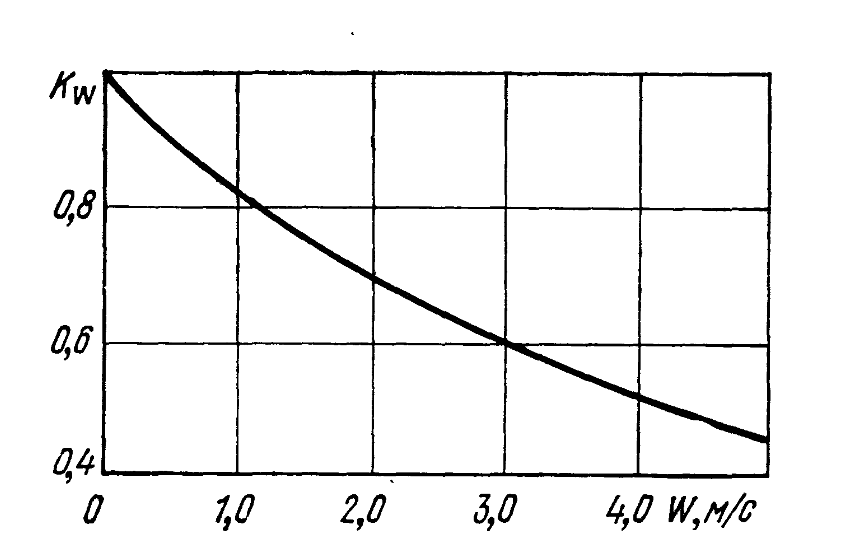
\includegraphics[scale=0.5]{images/Rotkop_pic_4.10.png}
  \caption{Зависимость $K_W$ от скорости
перемешивания~\cite{Rotkop1976}. }
\end{figure}

\item Определяется перегрев корпуса блока:
$$\vartheta\mathrm{_к} = 17,3 K$$
\item Определяется перегрев нагретой зоны \cite{Rotkop1976}:
  \begin{equation}
    \vartheta\mathrm{_з} = \vartheta_1 \cdot (K\mathrm{_{Н1}} - 1) + \vartheta_2 K_w
  \end{equation}
$$    \vartheta\mathrm{_з} = 42,032 K$$

\item Определяется средний перегрев воздуха в блоке ~\cite{Rotkop1976}:
  \begin{equation}
    \vartheta\mathrm{_в} = 0,75 \cdot \vartheta\mathrm{_з}
  \end{equation}

  $$\vartheta\mathrm{_в} = 31,524K$$
\item Находится удельная мощность элемента~\cite{Rotkop1976}:
  $$q\mathrm{_{эл}} =1109,50966\mathrm{ВТ/м^2} $$
\item Рассчитывается перегрев поверхности элемента ~\cite{Rotkop1976}:
  $$\vartheta\mathrm{_{эл}} =59,218$$

\item Рассчитывается перегрев окружающей элемент среды ~\cite{Rotkop1976}:
  $$\vartheta\mathrm{_{эс}} = 44,414K $$
  
\item Находится температура корпуса блока ~\cite{Rotkop1976}:
  $$T\mathrm{_{к}} = 330,3 K$$
\item Находится температура нагретой зоны, поверхности элемента,
    средняя температура в блоке и температура окружающей среды:
    $$T\mathrm{_з} = 355,032 K$$
    $$T\mathrm{_{эл}} = 344,524 K$$
    $$T\mathrm{_{в}} = 372,218 K$$
    $$T\mathrm{_{эс}} =357,414 K$$

    
\end{enumerate}

\subsection{Расчет теплового режима РЭС в герметичном корпусе с наружным обдувом}

\begin{enumerate}[label={\arabic*.}]
\item Рассчитывается поверхность корпуса блока: % (4.46)
  $$S\mathrm{_{К}}=1,108\mathrm{м^2}$$

\item Рассчитывается условная поверхность нагретой зоны: % (4.39)
  $$S\mathrm{_{з}} = 0,655\mathrm{м^2}$$ 
\item Находится удельная мощность корпуса блока:  % (4.45)
  $$q\mathrm{_к} = 13,53\mathrm{Вт/м^2}$$

\item Находится удельная мощность нагретой зоны: % (4.38)
  $$q\mathrm{_з} = 22,91 \mathrm{ Вт/м^2}$$

\item Определяется коэффициент $\vartheta_1$ в зависимости от удельной мощности корпуса блока ~\cite{Rotkop1976}:

  $$\vartheta_1=1,938$$
\item Определяется коэффициент $\vartheta_2$ в зависимости от удельной мощности нагретой среды ~\cite{Rotkop1976}:
  $$\vartheta_2=3,182$$
  

\item Коэффициент $K\mathrm{_{Н2}}$ в зависмости от давления
  среды вне корпуса блока берётся из ГОСТ~\cite{GOST-15150-69}.

  $$K\mathrm{_{Н1}} = 0,996$$

\item Рассчитывается перегрев между нагретой зоной и корпусом блока
  ~\cite{Rotkop1976}:
  \begin{equation}
    \vartheta_{21} = (\vartheta_{2}-\vartheta_{1})K\mathrm{_{Н2}}
    \end{equation}

    $$\vartheta_{21}=1,240 K$$

\item Рассчитывается перегрев корпуса блока с наружным обдувом
    ~\cite{Rotkop1976}:
    \begin{equation}
      \vartheta\mathrm{_к} = q\mathrm{_к}/(12 + 4,17 \nu)
      \end{equation}
      \nu — скорость обдува. Принятая равной $5\mathrm{м/с}$,
      как близкая к среднему значению скорости ветра бытового
вентилятора.

$$\vartheta\mathrm{_к} = 0,698$$

\item Определим прегрев нагретой зоны блока с наружным обдувом
  ~\cite{Rotkop1976}:
  \begin{equation}
    \vartheta\mathrm{_з} =  \vartheta\mathrm{_к} + \vartheta_{21}
    \end{equation}
  
$$\vartheta\mathrm{_з} = 1,937$$

\item Определяется средний перегрев воздуха в блоке ~\cite{Rotkop1976}:
  \begin{equation}
    \vartheta\mathrm{_в} = 0,75 \cdot \vartheta\mathrm{_з}
  \end{equation}

  $$\vartheta\mathrm{_в} = 2,727$$
  \item Находится удельная мощность элемента~\cite{Rotkop1976}:
  $$q\mathrm{_{эл}} =73,934\mathrm{ВТ/м^2} $$
\item Рассчитывается перегрев поверхности элемента ~\cite{Rotkop1976}:
  $$\vartheta\mathrm{_{эл}} =3,016K$$

\item Рассчитывается перегрев окружающей элемент среды ~\cite{Rotkop1976}:
  $$\vartheta\mathrm{_{эс}} = 2,260K$$

\item Находится температуры корпуса блока, нагретой зоны, поверхности
  элемента, средняя температура в блоке и температура окружающей среды:
  $$T\mathrm{_{к}} = 313,697 K$$
  
    $$T\mathrm{_з} = 314,937 K$$
    $$T\mathrm{_{эл}} = 316,016 K$$
    $$T\mathrm{_{в}} = 314,453 K$$
    $$T\mathrm{_{эс}} =315,262 K$$

\end{enumerate}


\subsection{Расчет теплового режима РЭС в герметичном оребрённом
  корпусе}
\begin{enumerate}[label={\arabic*.}]

\item Рассчитывается поверхность неоребренного корпуса
  блока~\cite{Rotkop1976}: % (4.46)
  $$S\mathrm{_{К}}=1,108\mathrm{м^2}$$

\item Рассчитывается условная поверхность нагретой
  зоны~\cite{Rotkop1976}: % (4.39)
  $$S\mathrm{_{з}} = 0,655\mathrm{м^2}$$ 

\item Находится удельная мощность корпуса
  блока ~\cite{Rotkop1976}:  % (4.45)
  $$q\mathrm{_к} = 13,53\mathrm{Вт/м^2}$$

\item Находится удельная мощность нагретой
  зоны: % (4.38)
  $$q\mathrm{_з} = 22,91 \mathrm{ Вт/м^2}$$

\item Определяется коэффициент $\vartheta_1$ в зависимости от
  удельной мощности корпуса блока:

  $$\vartheta_1=1,938$$
\item Определяется коэффициент $\vartheta_2$ в зависимости от удельной мощности нагретой среды:
  $$\vartheta_2=3,182$$

\item Рассчитывается прегрев мужду нагретой зоной и корпусом
неоребренного блока

$$\vartheta_{21} = 1,24 K$$

\item Рассчитывается поверхность оребренного корпуса блока,
  как сумму поверхности блока и поверхности корпуса:
  \begin{equation}
    S\mathrm{_{кр}} = S\mathrm{_{кн}} + S_{p}
  \end{equation}

Суть добавления рёбер в данном случае заключается в увелечении площади
рассеивания. Возьмём площадь рёбер равной четверти от площади
корпуса. Тогда:
$$S\mathrm{_{кр}} = S\mathrm{_{кр}} \cdot 1,25 = 1,386$$

\item Рассчитаем удельную мощность оребренного
  корпуса блока~\cite{Rotkop1976}:
  \begin{equation}
      q\mathrm{_{кр}} = P\mathrm{_{з}} / S\mathrm{_{кр}}
    \end{equation}
    
    $$q\mathrm{_{кр}} = 10,826 \mathrm{Вт/м^2}$$

\item
    Определим коэффициент $\vartheta_{1p}$ в зависимости от удельной
    мощности оребрённого корпуса блока~\cite{Rotkop1976}:

\begin{equation}
\vartheta_{1p} = 0,1472q\mathrm{_{кр}} - 0,2962 \cdot 10^{-3}q\mathrm{_{кр}}^2 + 0,3127 \cdot 10^{-6}q\mathrm{_{кр}}^2      
\end{equation}

$$\vartheta_{1p}= 1,559K$$

\item Коэффициент $K\mathrm{_{Н1}}$ в зависмости от давления
  среды вне корпуса блока берётся из ГОСТ~\cite{GOST_15150-69}.

  $$K\mathrm{_{Н1}} = 0,999$$


\item Коэффициент $K\mathrm{_{Н2}}$ в зависмости от давления
  среды внутри корпуса блока берётся из ГОСТ~\cite{GOST_15150-69}.

  $$K\mathrm{_{Н2}} = 0,999$$

\item Рассчитывается перегрев оребренного корпуса блока
  \begin{equation}
    \vartheta\mathrm{_к} =\vartheta{_{1p}}K\mathrm{_{H1}}
  \end{equation}

  $$\vartheta\mathrm{_к} = 1,557K$$

\item Рассчитывается
  перегрев нагретой зоны
  с оребренным корпусом ~\cite{Rotkop1976}:

\begin{equation}
    \vartheta\mathrm{_з} = \vartheta{_к} +(\vartheta_2 - \vartheta_1)K\mathrm{_{Н2}}
  \end{equation}
  $$\vartheta\mathrm{_з} = 2,801K$$

\item Рассчитывается средний прогрев воздуха в блоке
  \begin{equation}
    \vartheta\mathrm{_в} = 0,75 \cdot \vartheta\mathrm{_з}
  \end{equation}
  
  $$\vartheta\mathrm{_в} = 2,1K$$

\item Определяется удельная мощность элемента, перегревы его
    поверхности и окружающей среды:
    $$q\mathrm{_{эл}} =73,93$$
    $$\vartheta\mathrm{_{эл}} = 53,87 K$$

    $$\vartheta\mathrm{_{эс}} = 4,359 K$$

  \item Находятся температуры поверхности корпуса блока, нагретой
зоны, поверхности элемента, воздуха в блоке и окружающей элемент
среды:
$$T\mathrm{_{к}} = 314,557 K$$
$$T\mathrm{_з} = 315,801 K$$
$$T\mathrm{_{эл}} = 315,100 K$$
$$T\mathrm{_{в}} = 366,875 K$$
$$T\mathrm{_{эс}} =317,36 K$$

\end{enumerate}

\subsection{Расчет теплового режима РЭС в перфорированном корпусе}

\begin{enumerate}[label={\arabic*.}]

\item Рассчитывается:
  поверхность корпуса блока,
  условная поверхность нагретой зоны,
  удельная мощность корпуса блока,
  удельная мощность нагретой зоны.

  $$S\mathrm{_{К}}=1,108\mathrm{м^2}$$
  $$S\mathrm{_{з}} = 0,655 \mathrm{м^2}$$
  $$q\mathrm{_к} = 13,53\mathrm{Вт/м^2}$$
  $$q\mathrm{_з} = 22,91 \mathrm{ Вт/м^2}$$

\item Находятся коэффициенты $\vartheta_1$ и
  $\vartheta_2$ в зависимости от
  удельной мощности корпуса блока и
  удельной мощности нагретой зоны.

  $$\vartheta_1=1,936$$
  $$\vartheta_2=3,122$$


\item Коэффициенты $K\mathrm{_{Н1}}$ и $K\mathrm{_{Н2}}$
  в зависимости от давления вне и
  внутри корпуса блока берутся из ГОСТ

  $$K\mathrm{_{Н1}} = 0,999$$
  $$K\mathrm{_{Н1}} = 0,996$$

\item Рассчитывается площадь (круглых)
  перфорационных отверстий~\cite{Rotkop1976}:
  \begin{equation}
    S = \frac{n \cdot \pi \cdot d^2}{4}
    \end{equation}
    Здесь n — количество отверстий $n = 60$,
    d – диаметр отверстия $d = 0,00635\mathrm{м}$.

    $$S = 0,00380\mathrm{м^2}$$

\item Рассчитывается коэффициент перфорации
    как отношение площади перфорации к
    площади основания корпуса ~\cite{Rotkop1976}:
    \begin{equation}
    \mathrm{П} = S\mathrm{_п}/2 l_1 l_2
  \end{equation}

  $$\mathrm{П} = 0,00981$$

\item Находится коэффициент $K\mathrm{_П}$ в зависимости от
  коэффициента перфораций:
  \begin{equation}
    K\mathrm{_П} = 0,29 + \frac{1}{1,41 + 4,95}
  \end{equation}
 
  $$K\mathrm{_П} = 0,976$$

\item Определяется прегрев корпуса блока~\cite{Rotkop1976}:
  \begin{equation}
    \vartheta\mathrm{_К} = \vartheta_1K\mathrm{_{Н1}}K\mathrm{_П} \cdot 0,93
  \end{equation}

  $$\vartheta\mathrm{_К} =1,755K$$

\item Определяется перегрев нагретой зоны~\cite{Rotkop1976}:
  \begin{equation}
\vartheta\mathrm{_з} = 0,93К\mathrm{_п}(\vartheta_1K\mathrm{_{Н1}} + (\vartheta_2\frac{1}{0,93} - \vartheta_1)K\mathrm{_{Н2}})
\end{equation}

$$\vartheta\mathrm{_з} = 3,039 K$$

\item Определяется средний перегрев воздуха вблоке~\cite{Rotkop1976}:
\begin{equation}
\vartheta\mathrm{_в} = \vartheta\mathrm{_з} \cdot 0,6
\end{equation}

$$\vartheta\mathrm{в} = 1,823 K$$


\item Рассчитывается удельная мощность элемента,
  перегрев поверхности элемента,
  перегрев окружающей элемент среды:

$$q\mathrm{_{эл}}= 221,803\mathrm{ВТ/м^2}$$

$$\vartheta\mathrm{_{эл}} = 7,934K$$

$$\vartheta\mathrm{_{эс}} = 5,95$$

\item Находятся температуры
  корпуса блока,
  нагретой зоны,
  поверхности элемента,
  воздуха в блоке,
  окружающей элемент среды:

  
$$T\mathrm{_К} = 314,755$$

$$T\mathrm{_з} = 318,346$$

$$T\mathrm{_{эл}} = 324,243$$

$$T\mathrm{_{в}} = 316,208$$

$$T\mathrm{_{эс}} = 319,746$$


\end{enumerate}

\subsection{Расчет теплового режима РЭС при принудительном воздушном охлаждении}

Для расчетов был выбран вентилятор от производитля \textit{5bites}
\textit{FB5010S-12L3} c диаметром лопастей 45мм.

\begin{enumerate}[label={\arabic*.}]
\item Определяется средний перегрев воздуха в блоке
\begin{equation}
\vartheta\mathrm{_в} = 5 \cdot 10^{-4} \cdot \frac{P}{G}
\end{equation}

Здесь G – воздушный поток, а P мощность рассеиваемая элементом.

$$G = 0,06377\mathrm{м^3/c}$$

$$P = 20\mathrm{Вт}$$

$$\overline{\vartheta\mathrm{_в}} = 0,156K$$  
\item Определяется площадь поперечного
  в направлении продува сечения корпуса блока $$S= L_1 \cdot L_2$$,
  где $L_1$, $L_2$ — размеры корпуса блока,
  перпендикулярные направлению продува.
  $$S= L_1 \cdot L_2 =0,27\mathrm{м^2}$$

\item Находится коэффициент $m_1$ в зависимости
  от массового расхода охлаждающего воздуха ~\cite{Rotkop1976}:
  \begin{equation}
    m_1 = 0,001 \cdot G^{-0,5}
    \end{equation}
  $$m_1 = 0,0039$$

\item Находится коэффициент $m_2$,
  учитывающий величину площади поперечного
  к направлению обдува сечения аппарата\cite{Rotkop1976}:
  \begin{equation}
    m_2= (L_1 \cdot L_2) ^ {-0,406}
    \end{equation}

    $$m_2 = 1,7$$

  \item Находится коэффицент $m_3$,
    учитывающий длину аппарата в направлении обдува~\cite{Rotkop1976}:
    \begin{equation}
      m_3 = l_3 ^ {-1,059}
      \end{equation}

      $$m_3 = 4,269$$

\item Находится коэффициент $m_4$,
   учитывающий заполнение аппарата ~\cite{Rotkop1976}:
   \begin{equation}
     m_4 = K\mathrm{_{з}}^{-0,42}(1-K\mathrm{_{з}}^{2/3})^{0,5}
   \end{equation}
   $$m_4 = 1,595$$
  
\item Находится перегрев охлаждающего воздуха
  в радиоэлектронном аппарате ~\cite{Rotkop1976}:
  \begin{equation}
    \overline{\vartheta\mathrm{_{в}}} = 5 \cdot 10^{-4} P/G
  \end{equation}
  
  $$\overline{\vartheta\mathrm{_{в}}} = 0,157K$$

\item Рассчитывается перегрев нагретой зоны блока с принудительным

  охлаждением ~\cite{Rotkop1976}:
  \begin{equation}
    \vartheta\mathrm{_{з}} = \overline{\vartheta\mathrm{_{в}}} + P m_1 m_2 m_3 m_4
    \end{equation}
  

    $$\overline{\vartheta\mathrm{_{з}}} = 1,073 K$$

\item Находится условная поверхность нагретой зоны:
  $$S\mathrm{_{з}} = 0,654 \mathrm{м^3}$$

\item Находится удельная мощность нагретой зоны:
  $$q\mathrm{_{з}} = 22,1$$

\item Находится удельная мощность элемента:
  $$q\mathrm{_{эл}} = 73,93$$

\item Рассчитывается перегрев поверхности элемента ~\cite{Rotkop1976}
    \begin{equation}
    \vartheta\mathrm{_{эл}}   =  \vartheta\mathrm{_{з}} (0,75 + 0,25\frac{q\mathrm{_{эл}}}{q\mathrm{_{з}}} (\frac{L}{L_{3}} + 0,5)
    \end{equation}

    $$\vartheta\mathrm{_{эл}} = 5,841$$

\item Рассчитывается перегрев окружающей
  среды у элемента ~\cite{Rotkop1976}:
  \begin{equation}
    \vartheta\mathrm{_{эс}}   =  \vartheta\mathrm{_{в}} (0,75 + 0,25\frac{q\mathrm{_{эл}}}{q\mathrm{_{з}}} (\frac{L}{L_{з}})
    \end{equation}
  
  $$\vartheta\mathrm{_{эс}} = 0,854 K$$

\item Определяется температура нагретой зоны ~\cite{Rotkop1976}:
  \begin{equation}
    T\mathrm{_{з}} = \vartheta\mathrm{_{з}} + T\mathrm{_{вх}}
  \end{equation}

  $$T\mathrm{_{з}} = 314,073K$$
  
\item Определяется средняя температура воздуха в блоке ~\cite{Rotkop1976}:
  \begin{equation}
    T\mathrm{_{в}} = \overline{\vartheta\mathrm{_{в}}} + T\mathrm{_{вх}}
  \end{equation}
  
  $$ T\mathrm{_{в}} = 313,157K$$
 
\item Определяется температура воздуха на выходе из
  блока ~\cite{Rotkop1976}:
  \begin{equation}
    T\mathrm{в2} = 2\cdot \overline{\vartheta\mathrm{_{в}}} + T\mathrm{_{вх}}
  \end{equation}
  
  $$ T\mathrm{в2} = 313,314K$$
  
\item Определяется температура поверхности элемента ~\cite{Rotkop1976}:
  \begin{equation}
    T\mathrm{_{эл}} = \vartheta\mathrm{_{эл}}  + T\mathrm{_{вх}}
  \end{equation}
  $$    T\mathrm{_{эл}} = 314,188K$$
  
\item Определяется температура окружающего
  элемент воздуха ~\cite{Rotkop1976}:
  \begin{equation}
        T\mathrm{_{эc}} = \vartheta\mathrm{_{c}} + T\mathrm{_{вх}}
    \end{equation}

 $$    T\mathrm{_{эл}} = 313,174K$$

  
\end{enumerate}
\newpage % Конец второй главы


\section{Анализ полученных результатов теплового режима РЭС}
\subsection{Обработка и анализ данных проведенного результата}

Гораздо легче принимать конструкторские решения обладая визуальным
представлением данных. По это причине данный раздел в основном состоит
из гистогорамм отображающих в результаты расчетов температур.




\subsubsection{Анализ тепловых режимов для корпуса блока:}
\begin{figure}[h] %% h means here
\begin{center}
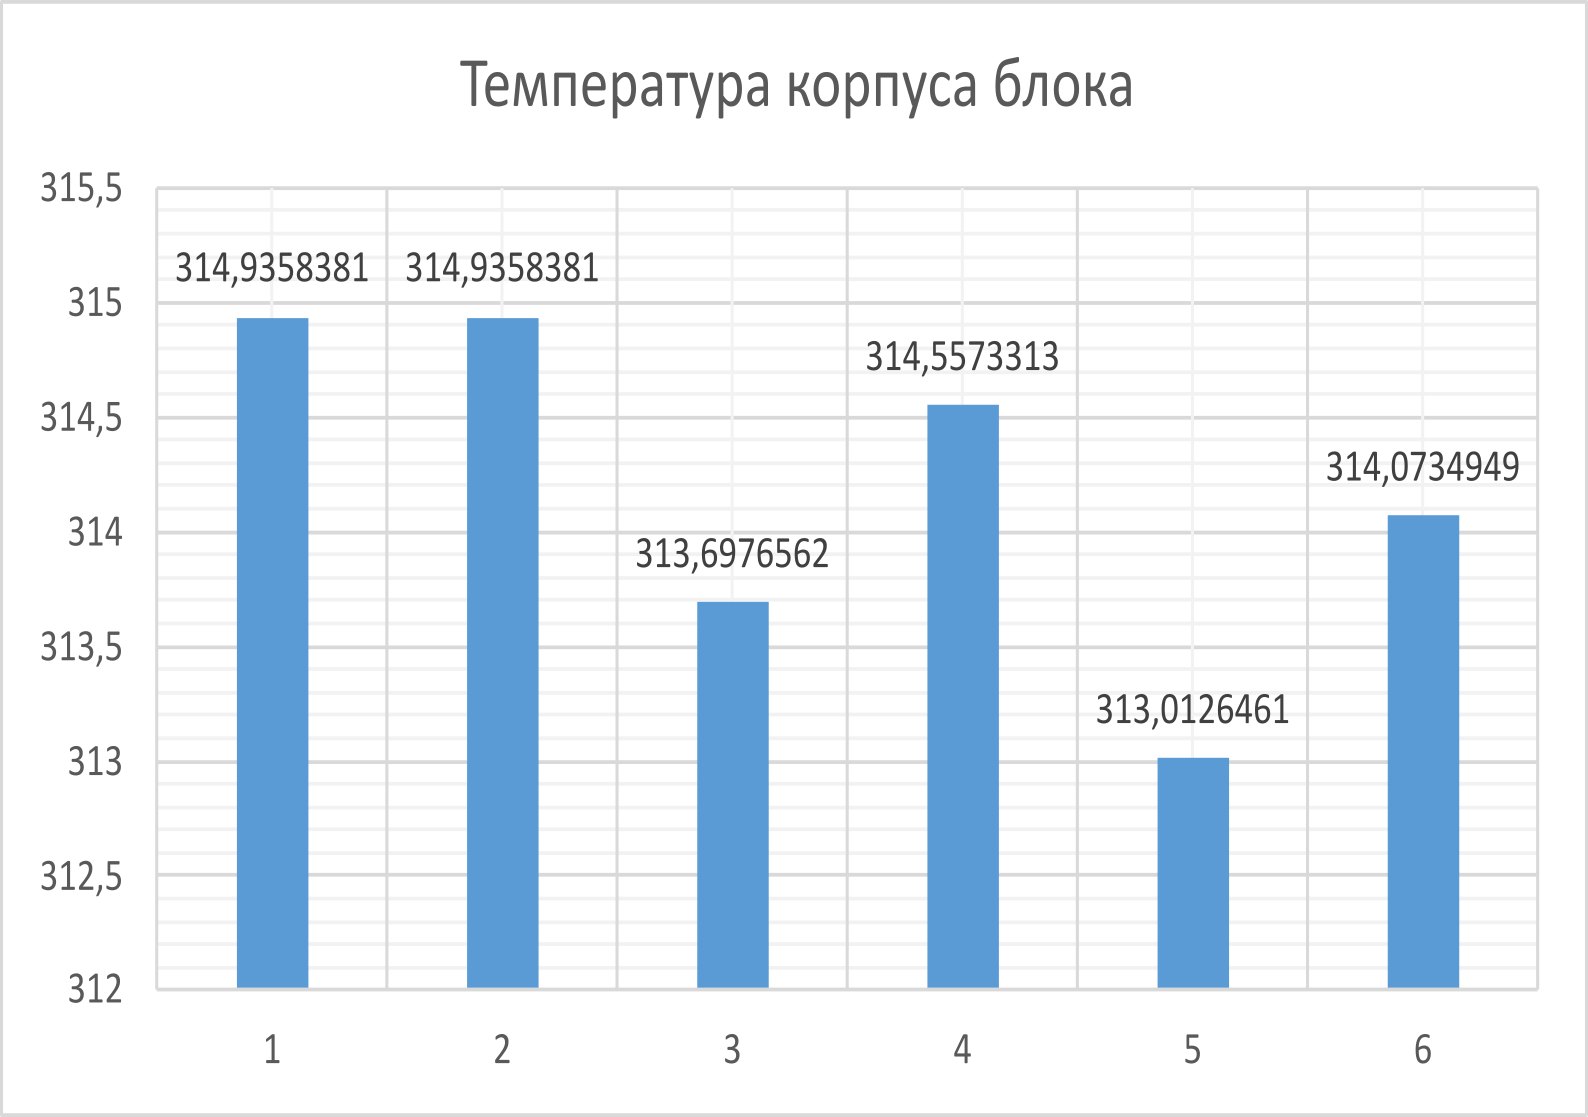
\includegraphics[scale = 0.4]{t_corp.png}
\caption{Температура корпуса блока:\\
  1 - тепловой режим герметичного корпуса\\
  2 – тепловой режим блока в герметичном корпусе с внутренним перемешиванием\\
  3 – тепловой режим блока в герметичном корпусе с наружным обдувом\\
  4 - телповой режим блока в  герметичном оребренном корпусе \\
  5 – тепловой режим блока в перфорированном корпусе \\
  6 - тепловой режим блока при принудительном охлаждении}
\end{center}

\end{figure}

На гистогорамме ожидаемо оказались равными значения температур для
герметичного корпуса и для корпуса с внутренним перемешиванием. Это
обусловлено тем, что скорость перемешивания при расчете была равна
нулю и закономерно.

Неожиданно то, что значения температур при принудительном и охлаждении
и при использовании оребренного корпуса оказались выше, нежели те же
значения для режима с обдувом и использовании перфорированного корпуса.

С другой стороны, можно обосновать низкую температуру корпуса при
обдуве тем, что при таком методе охлаждения набегающим потоком воздуха
тепло отводится в первую очередь от корпуса.

Самым эффективным оказалось использование перфорированного корпуса.
Это настораживает, так как принудительное охлаждение считается по
определению самым эффективным и поэтмум возникают вопросы
к правильности рассчета, когда самая низкая температура оказывается в
тепловом режиме с перфорированием.\\


\subsubsection{Анализ тепловых режимов для поверхности элемента:}
\begin{figure}[h] %% h means here
\begin{center}
  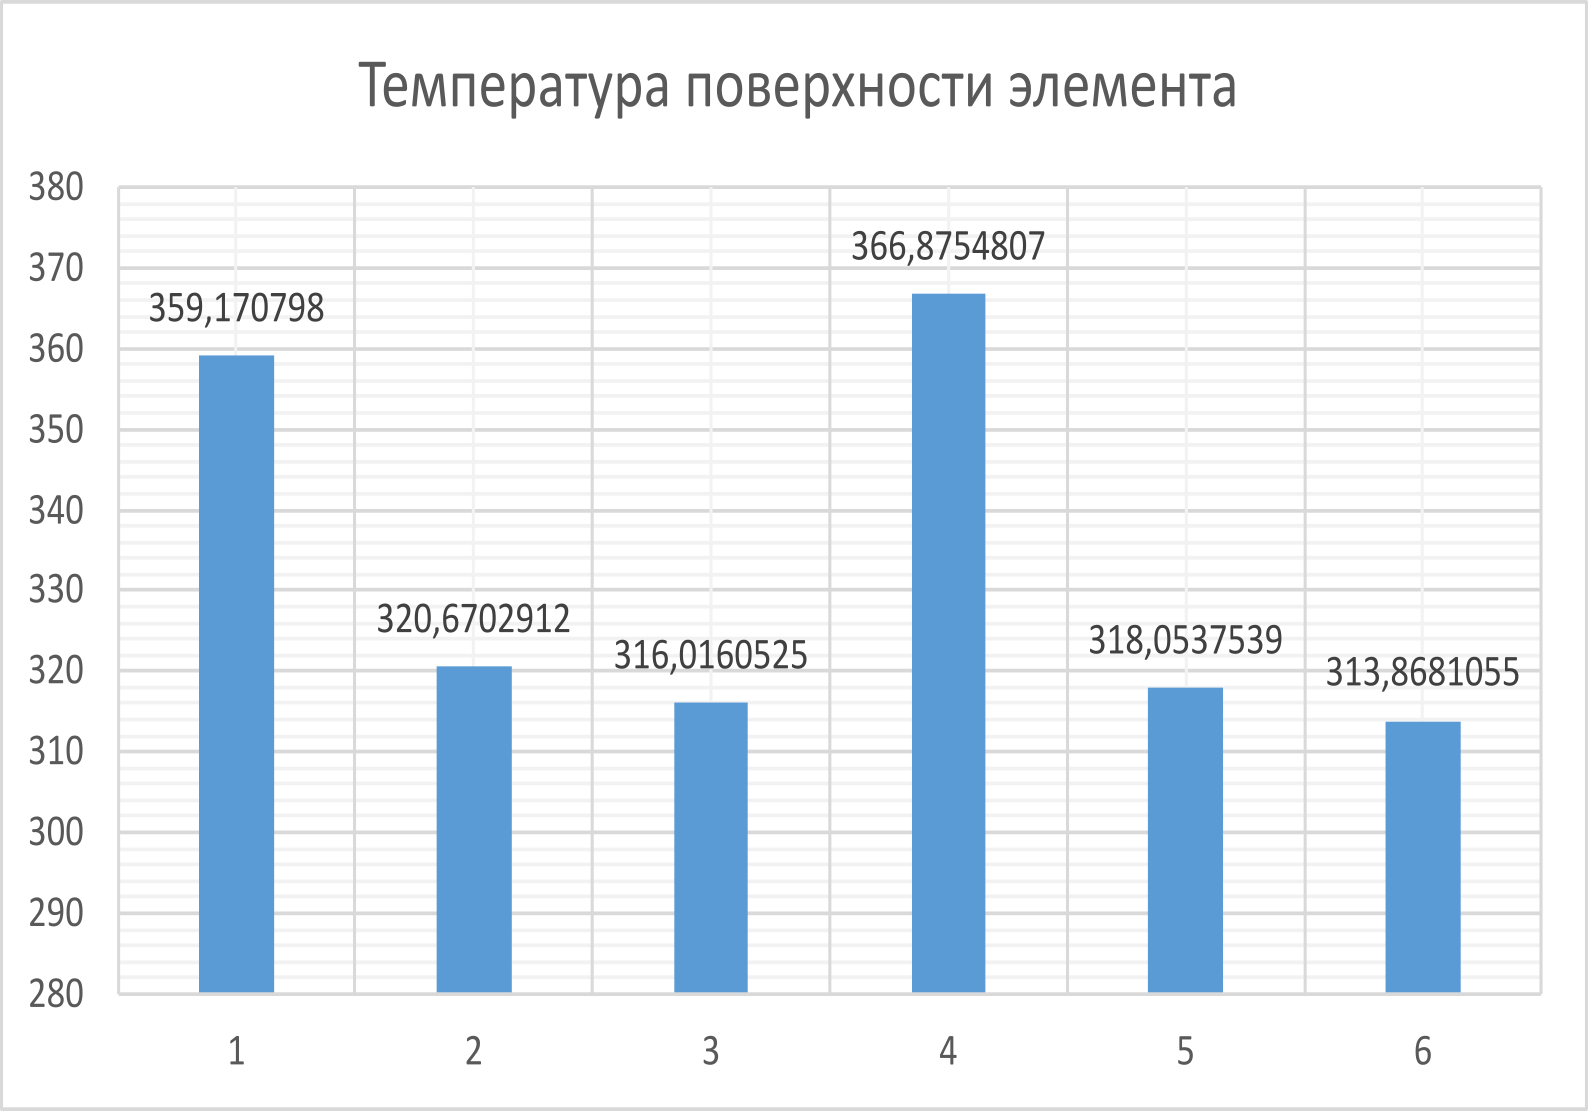
\includegraphics[scale = 0.4]{t_surface.png}
  \end{center}
\caption{Температура поверхности элемента:\\
  1 - тепловой режим герметичного корпуса\\
  2 – тепловой режим блока в герметичном корпусе с внутренним перемешиванием\\
  3 – тепловой режим блока в герметичном корпусе с наружным обдувом\\
  4 - телповой режим блока в  герметичном оребренном корпусе \\
  5 – тепловой режим блока в перфорированном корпусе \\
  6 - тепловой режим блока при принудительном охлаждении}

\end{figure}

Ожидаемое самым низким оказалась температура в телповом режими с
принудительным охлажденим.

Однако температура при расчете для
теплового режима блока в оребренном корпусе оказалось выше, даже чем
тепловой режим герметичного корпуса, что объяснить сложно. Это также
может свидетелсьтвовать об ошибках вычислениях.

\subsubsection{Анализ тепловых режимов для воздуха в блоке.}
\begin{figure}[h] %% h means here
\begin{center}
  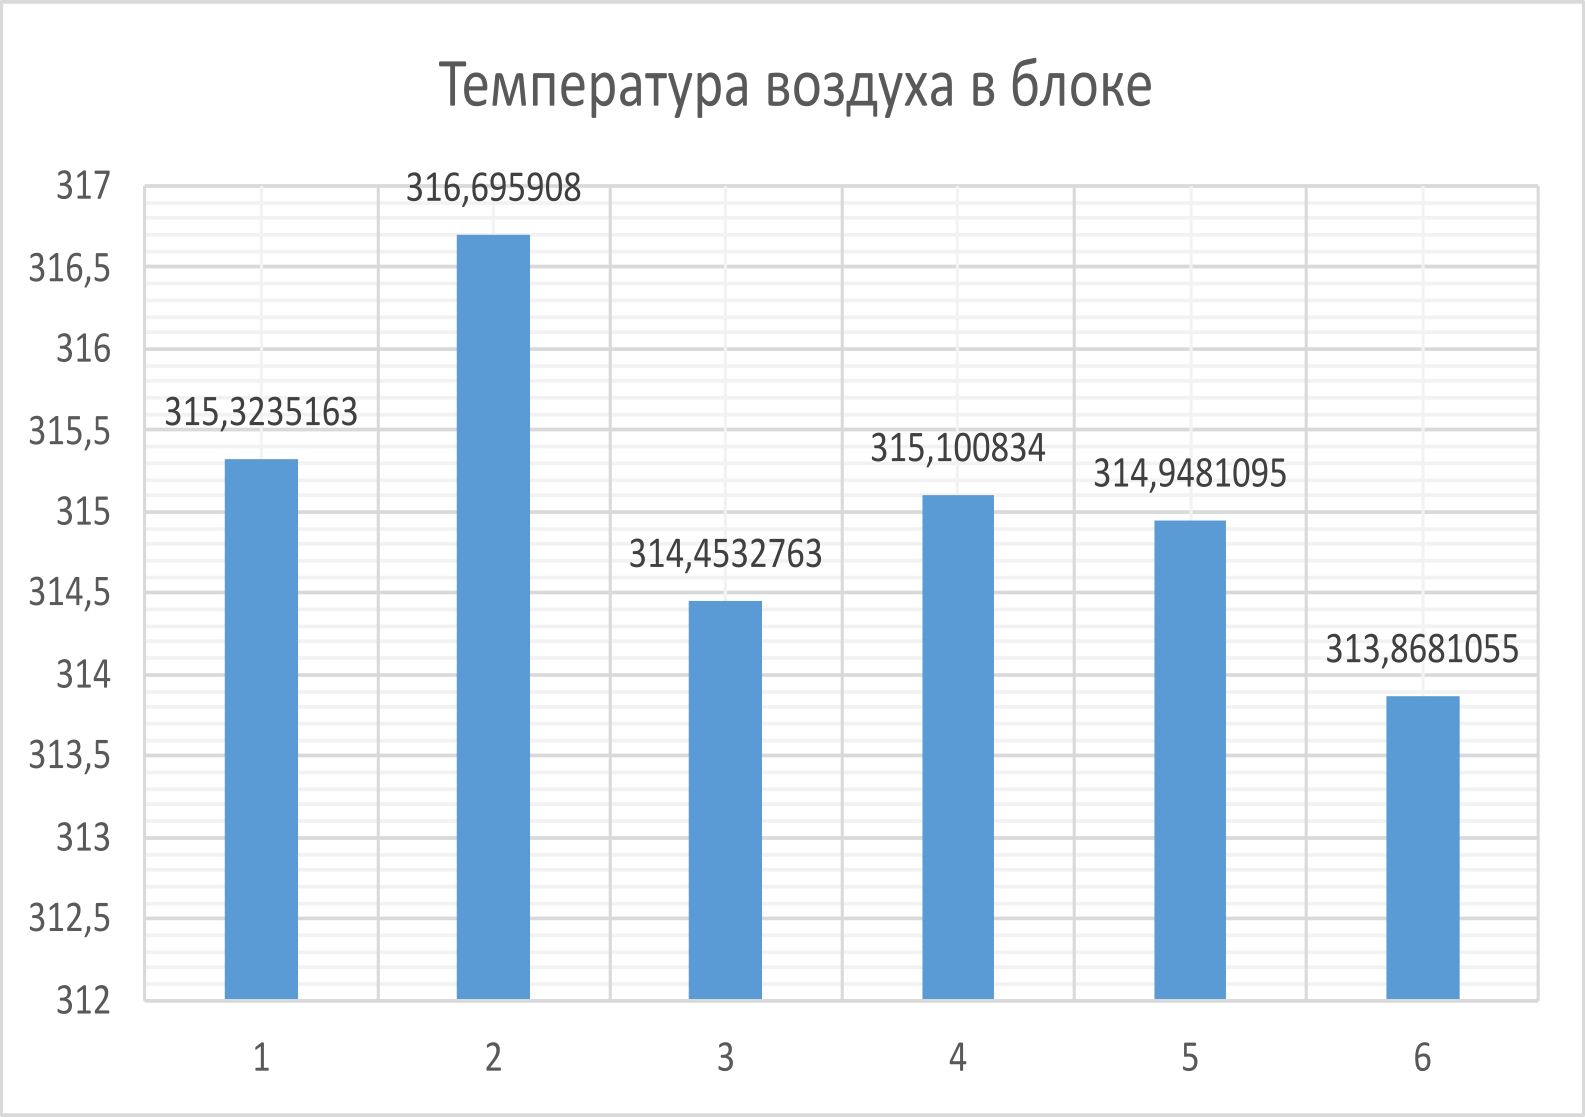
\includegraphics[scale = 0.4]{t_air.png}
  \end{center}
\caption{Температура воздуха блоке:\\
  1 - тепловой режим герметичного корпуса\\
  2 – тепловой режим блока в герметичном корпусе с внутренним перемешиванием\\
  3 – тепловой режим блока в герметичном корпусе с наружным обдувом\\
  4 - телповой режим блока в  герметичном оребренном корпусе \\
  5 – тепловой режим блока в перфорированном корпусе \\
  6 - тепловой режим блока при принудительном охлаждении}

\end{figure}

На данной графике самым эффективным оказывается режим с принудительным
воздушным охлажденим, что закономерно.

Однако, на графике видно, что при перемешивании температура воздуха выше,
чем при его отсуствие.

В прочем, сложно сказать достоверно ли это, так как при расчете
скорость перемешивания взята равной нулю, что обусловлено тем, что
охлаждение естественное.


На этом этапе становится анализа становятся очевидн
\begin{enumerate}[label={\arabic*.}]

\item Самое эффективный способ охлаждения из рассмотренных
  — принудительное воздушное охлаждение.
\item Значения первых двух тепловых режимов, то есть теплового режима
  герметичного корпуса и герметичного корпуса с перемешиванием в
  большинстве случаев будут выше чем значения в остальных температурных режимах.
  
\end{enumerate}

    Это означает, что более пристальному анализу подлежат только
    третий, четвёртый и пятый режимы,
    соответвенно обеспечивающие охлаждение

\subsubsection{ Анализ тепловых режимов окружающей элемент среды.}
\begin{figure}[h] %% h means here
\begin{center}
  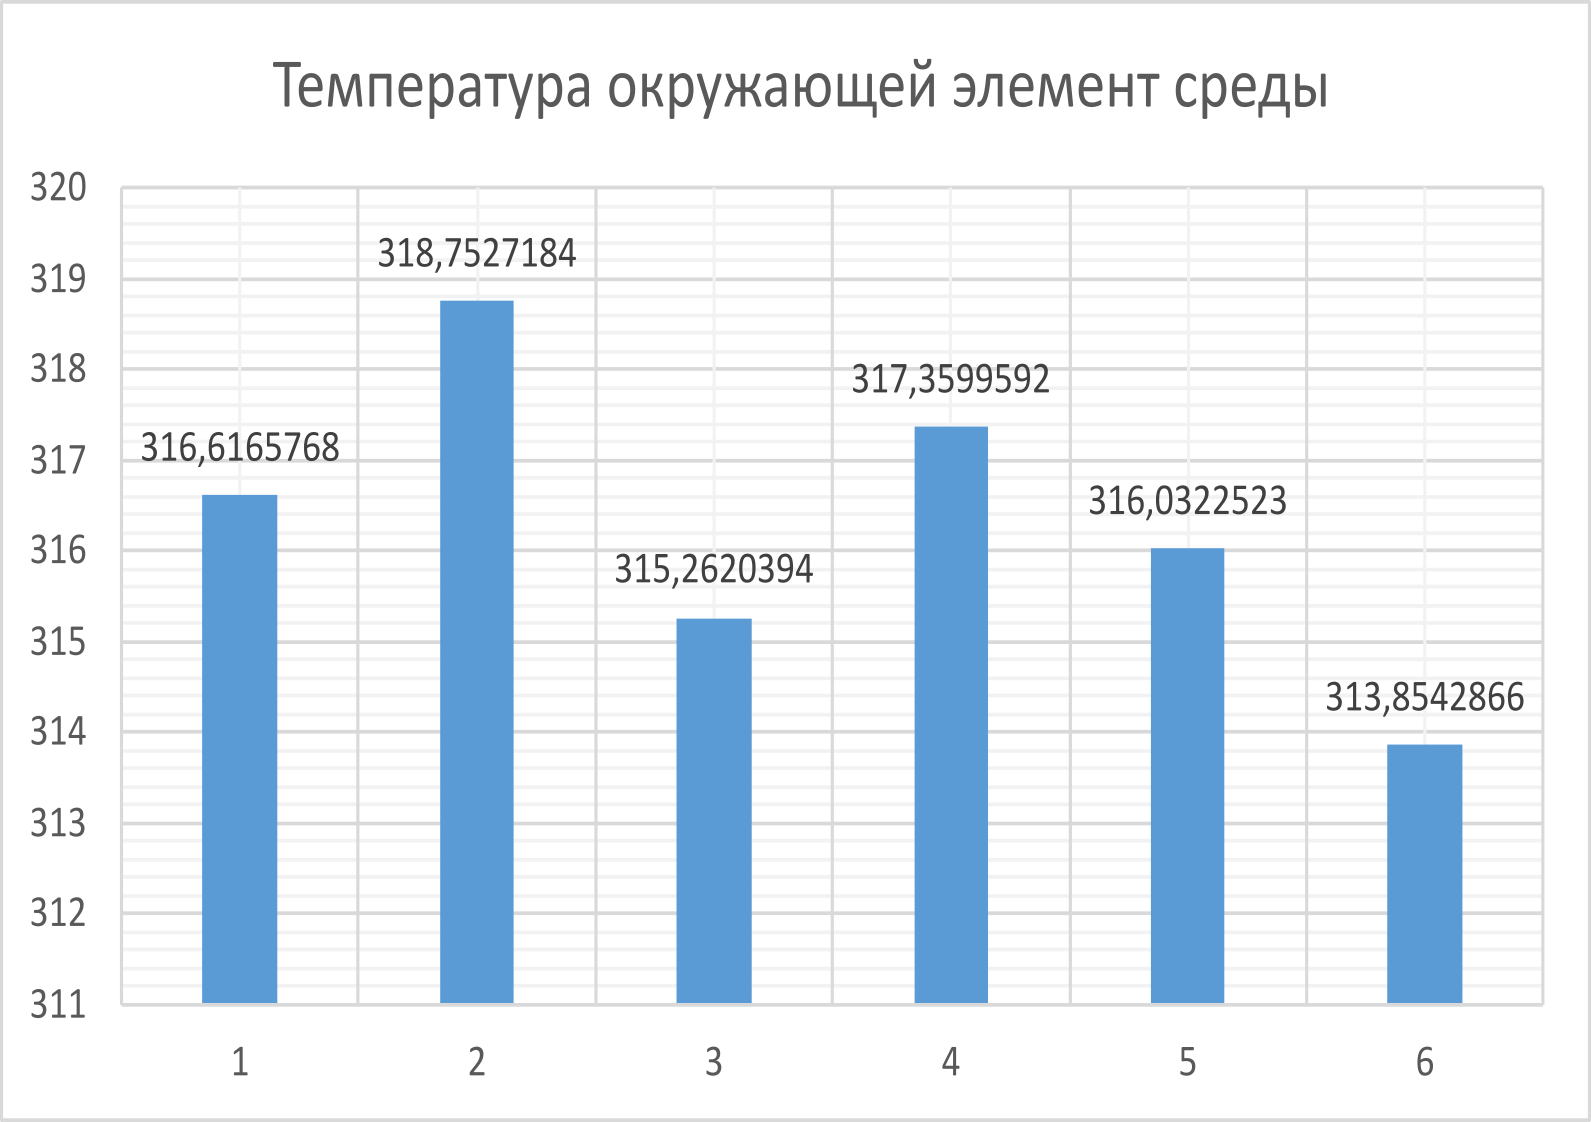
\includegraphics[scale = 0.4]{t_env.png}
  \end{center}
\caption{Температура окружающей элемент среды:\\
  1 - тепловой режим герметичного корпуса\\
  2 – тепловой режим блока в герметичном корпусе с внутренним перемешиванием\\
  3 – тепловой режим блока в герметичном корпусе с наружным обдувом\\
  4 - телповой режим блока в  герметичном оребренном корпусе \\
  5 – тепловой режим блока в перфорированном корпусе \\
  6 - тепловой режим блока при принудительном охлаждении}

\end{figure}

Данная гистограмма выглядит,
как наиболее близкая к действительным значениям,
если не учитывать разницу между тепловым режимом герметичного корпуса
и корпуса с перемешиваеним, при котором, в корпусе с перемешиваеним
оказывается большая температура.

\subsubsection{Анализ тепловых режимов  для
воздуха в блоке при способах охлаждения с помощью наружного обдува,
оребренным корпуса и перфорацией.}

\begin{figure}[h] %% h means here
\begin{center}
  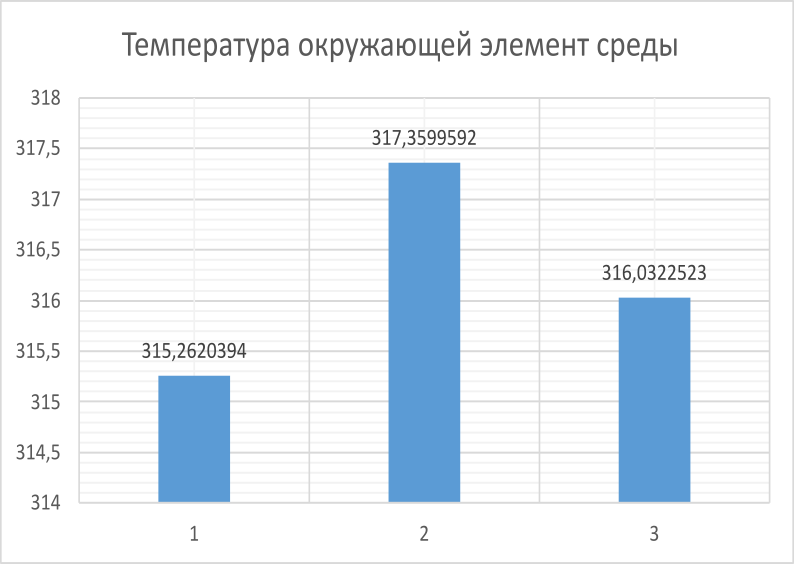
\includegraphics[scale = 0.4]{t_env_2.png}
  \end{center}
\caption{Температура воздуха в блоке:\\
  1 – тепловой режим блока в герметичном корпусе с наружным обдувом\\
  2 - телповой режим блока в  герметичном оребренном корпусе \\
  3 – тепловой режим блока в перфорированном корпусе \\
}

\end{figure}

На данной гистограмме видно, что наиболее эффективным из оставшихся
является охлаждение с наружным обдувом.

\subsubsection{Анализ тепловых режимов для окружающей элемент среды при
способах охлаждения с помощью наружного обдува, оребренным корпусом и
перфорацией.}

\begin{figure}[h] %% h means here
\begin{center}
  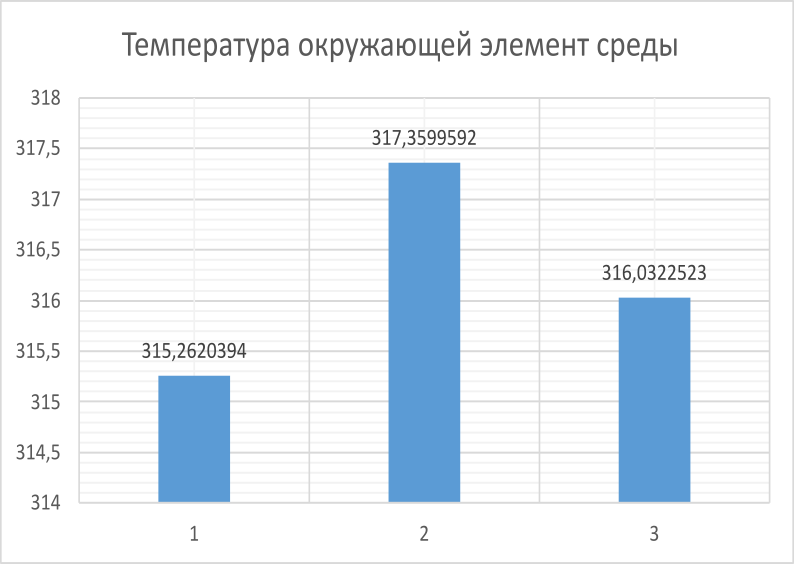
\includegraphics[scale = 0.4]{t_env_2.png}
\end{center}
\caption{Температура окружающей элемент среды:\\
  1 – тепловой режим блока в герметичном корпусе с наружным обдувом\\
  2 - телповой режим блока в  герметичном оребренном корпусе \\
  3 – тепловой режим блока в перфорированном корпусе \\
}

\end{figure}

Данная гистограмма также показывает охлажденим наружным обдувом как
самое эффективное.

На основании этого можно сделать заключение, что самым эфективным
после принудительного воздушного является метод охлаждения обдувом.
Конструкторами же устройства выбран метод охлаждения за счет
перфорации корпуса, который, является вторым по эффективности рассеивания тепла
и может быть предпочтительным.

\subsubsection{Моделирование теплового режима в elcut}

Было проведено моделирование печатной теплового режима печатной платы
в elcut.


\begin{figure}[h]
  \centering
  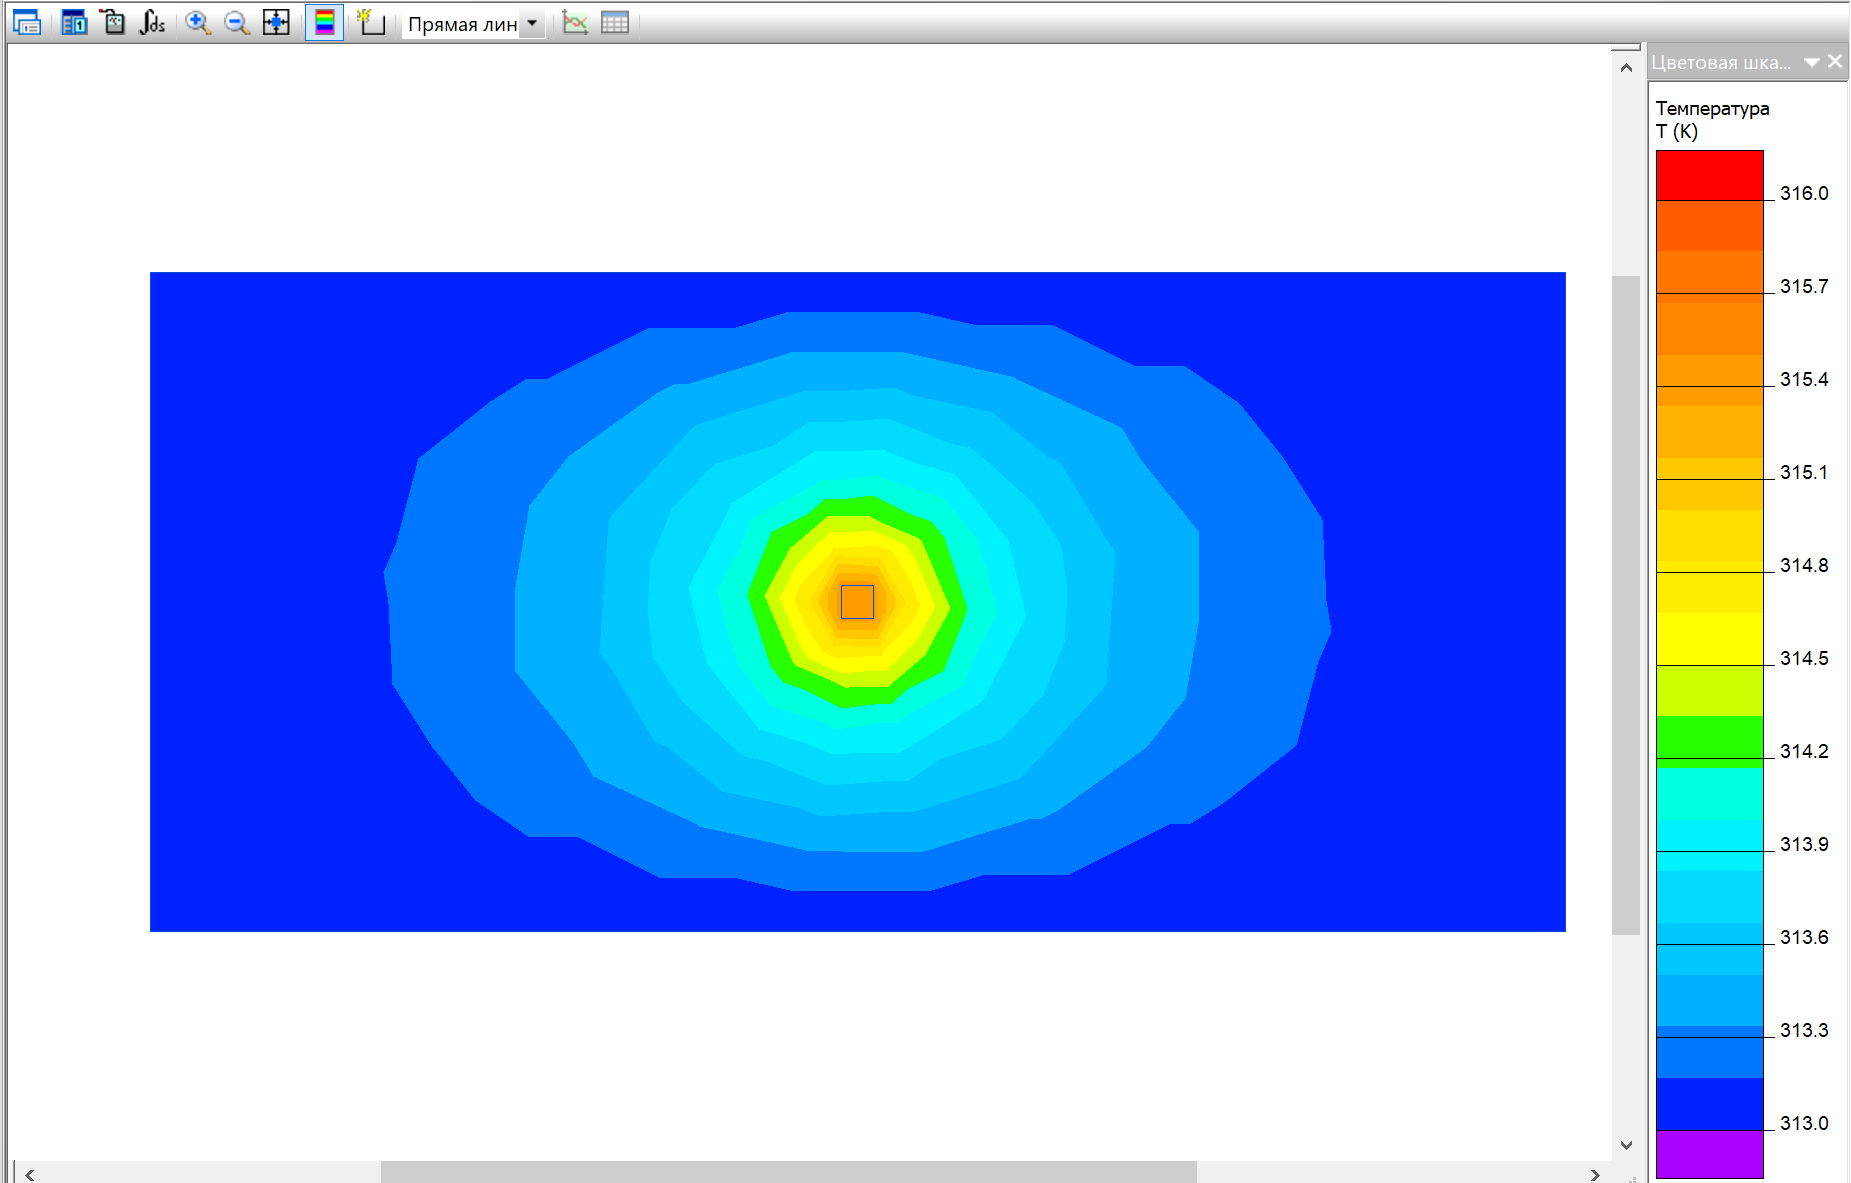
\includegraphics[scale = 0.30]{elcut_solved}
  \caption{
    Результат решения задачи теплопроводности в elcut. }
\end{figure}

В результате решения задачи тепловроднотси в elcut можно сделать
вывод, что за счет большой площади печатной платы происходит
рассеивание большей части тепловой энергии.

Это свидетельствует о том, что в данном конретном случае выбор
конкретного способа охлаждения не принципиален и использование не
самого эффективного его варианта, а именно использование корпуса с
охлажденим достаточно для решения задачи по обеспечению теплового
режима. 
%%% Третья глава
%\input{third_part}

\end{document}
